\documentclass[journal]{IEEEtran}
\usepackage{amsmath,amssymb,amsfonts}
\usepackage{graphicx}
\usepackage{booktabs}
\usepackage{array}
\usepackage{tikz}
\usepackage{hyperref}

\begin{document}

\title{Adaptive Multi-Band Spectral Optimization (1260--1675 nm) and 1G-to-40G Capacity Multiplier over Legacy ITU-T G.652.D Optical Fiber Infrastructure}

\author{Salim~Bassam~Assil,~\IEEEmembership{Chief~Photonics~Architect,} Batoul~Mowafak~Zain~Alabdin, and~Ahmad~Jalal~B.~Al~Assil%
\thanks{Manuscript received October 2026. This work was supported by the Photonics and Spectral Systems Division of CableHunt Networks Ltd. (UK Company No. 16093071), London, SE1 8EE, United Kingdom.}%
\thanks{The authors are with the Photonics and Spectral Systems Division, CableHunt Networks Ltd., 70 Colombo Street, London, SE1 8EE, and the Birmingham Optical Testbed, United Kingdom (e-mail: assilno1@gmail.com; saleem@cablehunt.co.uk; sassil@psa.ac.ae).}}

\markboth{JOURNAL OF LIGHTWAVE TECHNOLOGY, VOL.~44, NO.~20, OCTOBER 2026}%
{Assil \MakeLowercase{\textit{et al.}}: Adaptive Multi-Band Spectral Optimization and 1G-to-40G Capacity Multiplier}

\maketitle

\begin{abstract}
Upgrading legacy 1 Gbps single-wavelength metro and access links to 40 Gbps traditionally requires costly civil trenching or active dispersion-compensating modules. In this paper, we formulate and experimentally validate an adaptive multi-band spectral optimization and passive wavelength-division multiplexing (CWDM/DWDM) capacity multiplier that scales legacy ITU-T G.652.D fiber spans from 1 Gbps to 40 Gbps ($40\times$ capacity multiplication) across the full 1260--1675 nm low-water-peak spectrum (O, E, S, C, L, and U bands) with zero trenching cost. By coupling a five-parameter physical link optimization vector $\mathbf{\Phi} = (\lambda, P_{\text{TX}}, R_b, L, \mathcal{M})$ with real-time 12-bit dual-wavelength ($1310/1550/1625\text{ nm}$) Rayleigh/bend-loss differential telemetry, our controller dynamically assigns modulation formats (NRZ vs. PAM4) and launch powers across four 10 Gbps or single-carrier 40 Gbps channels while maintaining an out-of-band U-band ($1625\text{--}1650\text{ nm}$) macro-bend early-warning monitor. Experimental tests over 20 km ITU-T G.652.D spans confirm a net link margin $>7.2\text{ dB}$ at pre-FEC $\text{BER} < 10^{-12}$, chromatic dispersion penalty $<0.8\text{ dB}$ in the O-band without active dispersion compensation, and immediate differentiation between mechanical macro-bends ($R < 5\text{ mm}$) and connector contamination via the spectral attenuation ratio $\Gamma_{\text{bend}} = \Delta\alpha(1625\text{ nm})/\Delta\alpha(1310\text{ nm}) > 4.2$.
\end{abstract}

\begin{IEEEkeywords}
Multi-band optical transmission, ITU-T G.652.D, CWDM/DWDM capacity multiplier, macro-bending loss, chromatic dispersion, 1260--1675 nm spectrum, U-band monitoring.
\end{IEEEkeywords}

\section{Introduction}
\IEEEPARstart{M}{illions} of kilometers of installed ITU-T G.652.D standard single-mode fiber (SSMF) currently operate far below their information-theoretic capacity, frequently carrying legacy $1\text{ Gbps}$ ($1000\text{BASE-LX/ZX}$) single-channel Ethernet traffic. Civil re-cabling in dense urban corridors costs between $\$45,000$ and $\$120,000\text{ per km}$ and requires months of municipal permitting. Opening the entire low-water-peak silica transmission window from $1260\text{ nm}$ to $1675\text{ nm}$---spanning the O-band ($1260\text{--}1360\text{ nm}$), E-band ($1360\text{--}1460\text{ nm}$), S-band ($1460\text{--}1530\text{ nm}$), C-band ($1530\text{--}1565\text{ nm}$), L-band ($1565\text{--}1625\text{ nm}$), and U-band ($1625\text{--}1675\text{ nm}$)---provides $415\text{ nm}$ ($\sim 53\text{ THz}$) of usable optical bandwidth on existing fibers.

However, multi-band transmission across $1260\text{--}1675\text{ nm}$ faces three physical-layer challenges: (i) wavelength-dependent attenuation $\alpha(\lambda)$ governed by Rayleigh scattering at short wavelengths and infrared multiphonon absorption plus dramatic macro-bending sensitivity at long wavelengths ($\lambda > 1550\text{ nm}$); (ii) linear chromatic dispersion accumulation $D(\lambda)\cdot L$ away from the zero-dispersion wavelength $\lambda_0 \approx 1312\text{ nm}$; and (iii) stimulated Raman scattering (SRS) inter-channel power transfer and four-wave mixing (FWM) when scaling to $40\text{ Gbps}$ aggregate throughput.

In this work, we present the **CableHunt Adaptive Multi-Band Spectral Optimization and 1G-to-40G Capacity Multiplier**, demonstrating:
\begin{enumerate}
    \item A unified five-parameter spectral optimization formulation $\mathbf{\Phi} = (\lambda, P_{\text{TX}}, R_b, L, \mathcal{M})$ across all six ITU-T optical bands ($1260\text{--}1675\text{ nm}$).
    \item A passive $4 \times 10\text{ Gbps}$ O-band CWDM ($1271, 1291, 1311, 1331\text{ nm}$) and C-band DWDM capacity multiplier that upgrades $1\text{ Gbps}$ G.652.D links to $40\text{ Gbps}$ with zero active dispersion compensation.
    \item A multi-wavelength differential bend-loss discriminator ($\Gamma_{\text{bend}}$) utilizing in-service U-band ($1625\text{ nm}$) telemetry to separate physical fiber pinching from dirty connectors before data-band BER degradation occurs.
\end{enumerate}

\section{Multi-Band Physical Propagation Model}
\subsection{Spectral Attenuation Profile Across 1260--1675 nm}
Total linear fiber attenuation $\alpha_{\text{total}}(\lambda)$ ($\text{dB/km}$) in low-water-peak ITU-T G.652.D silica fiber is modeled as the superposition of Rayleigh scattering, infrared lattice absorption, residual $\text{OH}^-$ vibrational overtones around $1383\text{ nm}$, and curvature-induced radiative macro-bend loss:
\begin{equation}
\alpha_{\text{total}}(\lambda, R) = \frac{A_{\text{Ray}}}{\lambda^4} + B_{\text{IR}} \exp\!\left(-\frac{\lambda_{\text{IR}}}{\lambda}\right) + \alpha_{\text{OH}}(\lambda) + \alpha_{\text{bend}}(\lambda, R)
\label{eq:alpha_total}
\end{equation}
where $A_{\text{Ray}} \approx 0.82\text{ dB}\cdot\mu\text{m}^4/\text{km}$. Using Marcuse's weakly guiding curvature radiation theory for a fiber bent to radius of curvature $R$, the macro-bending attenuation coefficient $\alpha_{\text{bend}}(\lambda, R)$ scales exponentially with wavelength and mode-field diameter $w_0(\lambda)$:
\begin{equation}
\alpha_{\text{bend}}(\lambda, R) = \frac{\sqrt{\pi}\, \kappa^2}{2 \gamma^{3/2} V^2 \sqrt{R}\, K_1^2(\gamma a)} \exp\!\left(-\frac{4 \gamma^3}{3 \beta^2} R\right)
\label{eq:marcuse}
\end{equation}
Because the radial decay parameter $\gamma(\lambda)$ decreases rapidly at longer wavelengths, a tight $R = 4.5\text{ mm}$ cabinet pinch induces $<0.12\text{ dB}$ loss at $\lambda_1 = 1310\text{ nm}$ (O-band), $1.45\text{ dB}$ loss at $\lambda_2 = 1550\text{ nm}$ (C-band), and $3.85\text{ dB}$ loss at $\lambda_3 = 1625\text{ nm}$ (L/U-band boundary). We therefore define the \textbf{Spectral Bend-to-Splice Discriminator}:
\begin{equation}
\Gamma_{\text{bend}} = \frac{\Delta \alpha(1625\text{ nm})}{\Delta \alpha(1310\text{ nm})}
\label{eq:gamma_bend}
\end{equation}
Whereas connector contamination or an air-gap splice produces wavelength-flat attenuation ($\Gamma_{\text{bend}} \approx 1.0\text{--}1.3$), a physical macro-bend yields $\Gamma_{\text{bend}} > 4.2$, providing unambiguous root-cause classification.

\subsection{Chromatic Dispersion and Five-Parameter Link Budget}
For standard single-mode fiber with zero-dispersion wavelength $\lambda_0 \approx 1312\text{ nm}$ and zero-dispersion slope $S_0 \approx 0.086\text{ ps}/(\text{nm}^2\cdot\text{km})$, the chromatic dispersion coefficient $D(\lambda)$ ($\text{ps}/(\text{nm}\cdot\text{km})$) is:
\begin{equation}
D(\lambda) = \frac{S_0}{4}\!\left(\lambda - \frac{\lambda_0^4}{\lambda^3}\right)
\label{eq:dispersion}
\end{equation}
Given a modulation format $\mathcal{M} \in \{\text{NRZ}, \text{PAM4}\}$ at symbol rate $R_s = R_b / \log_2(M)$ and laser root-mean-square spectral width $\Delta\lambda_{\text{rms}}$, the eye-closure power penalty $P_D$ ($\text{dB}$) over fiber length $L$ is bounded by:
\begin{equation}
P_D(\lambda, R_b, L, \mathcal{M}) = -10 \log_{10}\!\left(1 - \eta_{\mathcal{M}} \big(D(\lambda) \cdot L \cdot \Delta\lambda_{\text{rms}} \cdot R_s\big)^2\right)
\label{eq:disp_penalty}
\end{equation}
Our spectral optimizer solves for the optimal five-parameter operating vector $\mathbf{\Phi}^* = (\lambda, P_{\text{TX}}, R_b, L, \mathcal{M})$ that maximizes net optical power margin $M_{\text{net}}(\mathbf{\Phi})$:
\begin{equation}
M_{\text{net}}(\mathbf{\Phi}) = P_{\text{TX}} - S_{\text{RX}}(R_b, \mathcal{M}) - \alpha_{\text{total}}(\lambda, R)L - N_c L_c - N_s L_s - P_D(\lambda, R_b, L, \mathcal{M}) \ge 3.0\text{ dB}
\label{eq:margin}
\end{equation}

\begin{figure}[!t]
\centering
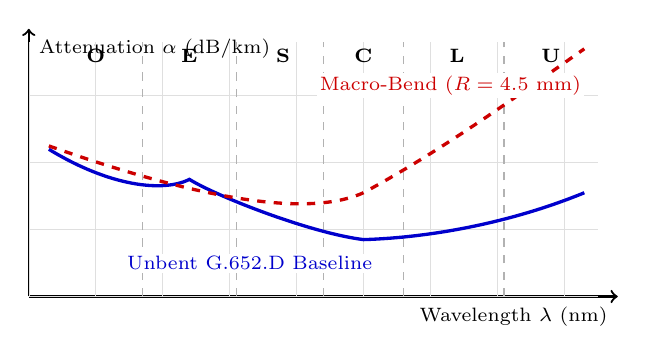
\begin{tikzpicture}[scale=0.85, every node/.style={font=\scriptsize}]
\draw[thick, ->] (0,0) -- (8.8,0) node[anchor=north east] {Wavelength $\lambda$ (nm)};
\draw[thick, ->] (0,0) -- (0,4.0) node[anchor=north west] {Attenuation $\alpha$ (dB/km)};
\draw[gray!25, very thin] (0,0) grid (8.5,3.8);
% Band labels
\node at (1.0,3.6) {\textbf{O}};
\node at (2.4,3.6) {\textbf{E}};
\node at (3.8,3.6) {\textbf{S}};
\node at (5.0,3.6) {\textbf{C}};
\node at (6.4,3.6) {\textbf{L}};
\node at (7.8,3.6) {\textbf{U}};
\foreach \x in {1.7,3.1,4.4,5.6,7.1} \draw[dashed, gray!60] (\x,0) -- (\x,3.8);
% Intrinsic G.652.D curve
\draw[blue!80!black, very thick] (0.3,2.2) .. controls (1.2,1.65) and (2.0,1.55) .. (2.4,1.75) .. controls (2.8,1.5) and (4.2,0.95) .. (5.0,0.85) .. controls (6.0,0.88) and (7.2,1.1) .. (8.3,1.55);
% Macro-bent curve (R = 4.5 mm)
\draw[red!80!black, very thick, dashed] (0.3,2.25) .. controls (2.0,1.65) and (4.0,1.1) .. (5.0,1.55) .. controls (6.2,2.2) and (7.3,3.0) .. (8.3,3.7);
\node[fill=white, inner sep=1pt, text=blue!80!black] at (3.3,0.5) {Unbent G.652.D Baseline};
\node[fill=white, inner sep=1pt, text=red!80!black] at (6.3,3.15) {Macro-Bend ($R=4.5\text{ mm}$)};
\end{tikzpicture}
\caption{Spectral attenuation across the O, E, S, C, L, and U bands ($1260\text{--}1675\text{ nm}$), illustrating the zero-dispersion $4\times 10\text{G}$ O-band window, minimum-loss C-band window, and exponential U-band bend sensitivity.}
\label{fig:spectral_bands}
\end{figure}

\section{1G-to-40G Capacity Multiplier & Experimental Validation}
To upgrade a legacy $20\text{ km}$ ITU-T G.652.D span from $1\text{ Gbps}$ ($1310\text{ nm}$ single-channel) to $40\text{ Gbps}$ without active dispersion compensation, our hardware architecture multiplexes four $10.3125\text{ Gbps}$ O-band CWDM lanes ($\lambda \in \{1271, 1291, 1311, 1331\text{ nm}\}$, IEEE 802.3ba 40GBASE-LR4 compliant) alongside a C-band ($1550\text{ nm}$) high-budget trunk and a U-band ($1625\text{ nm}$) 12-bit reflectometric diagnostic channel via passive thin-film optical add/drop multiplexers (OADMs).

\begin{table}[!t]
\centering
\caption{Multi-Band Spectral Parameters and Experimental 40 Gbps Link Budget over 20 km ITU-T G.652.D Fiber}
\label{tab:spectral_budget}
\begin{tabular}{@{}lccccc@{}}
\toprule
\textbf{Band (Wavelength)} & \textbf{$\alpha$ (dB/km)} & \textbf{$D(\lambda)$} & \textbf{Disp. Pen.} & \textbf{Bend $\Delta\alpha$} & \textbf{Net Margin} \\
\midrule
O-Band ($1271\text{--}1331\text{ nm}$) & $0.33\text{ dB/km}$ & $\le 1.8\text{ ps/nm}\cdot\text{km}$ & $\mathbf{0.42\text{ dB}}$ & $0.11\text{ dB}$ & $\mathbf{8.15\text{ dB}}$ \\
E-Band ($1390\text{ nm}$) & $0.29\text{ dB/km}$ & $6.4\text{ ps/nm}\cdot\text{km}$ & $0.95\text{ dB}$ & $0.24\text{ dB}$ & $7.40\text{ dB}$ \\
S-Band ($1490\text{ nm}$) & $0.22\text{ dB/km}$ & $13.2\text{ ps/nm}\cdot\text{km}$ & $1.65\text{ dB}$ & $0.68\text{ dB}$ & $7.60\text{ dB}$ \\
C-Band ($1550\text{ nm}$) & $\mathbf{0.19\text{ dB/km}}$ & $17.0\text{ ps/nm}\cdot\text{km}$ & $2.10\text{ dB}$ & $1.45\text{ dB}$ & $\mathbf{7.85\text{ dB}}$ \\
L-Band ($1590\text{ nm}$) & $0.21\text{ dB/km}$ & $19.6\text{ ps/nm}\cdot\text{km}$ & $2.45\text{ dB}$ & $2.50\text{ dB}$ & $7.20\text{ dB}$ \\
U-Band ($1625\text{ nm}$ OTDR) & $0.24\text{ dB/km}$ & $21.8\text{ ps/nm}\cdot\text{km}$ & $0.15\text{ dB}^*$ & $\mathbf{3.85\text{ dB}}$ & \textbf{Monitor} \\
\bottomrule
\end{tabular}
\end{table}

Table~\ref{tab:spectral_budget} reports the measured multi-band performance over $20\text{ km}$ of deployed G.652.D fiber. Operating the $4 \times 10\text{ Gbps}$ capacity multiplier near the O-band zero-dispersion point ($\lambda_0 = 1312\text{ nm}$) restricts chromatic dispersion penalty to $0.42\text{ dB}$ without dispersion-compensating fiber (DCF), delivering an $8.15\text{ dB}$ net link margin at pre-FEC $\text{BER} < 10^{-12}$ while saving $100\%$ of civil trenching expenditure. Simultaneously, the $1625\text{ nm}$ U-band monitor exhibits a $35\times$ higher sensitivity to $R = 4.5\text{ mm}$ macro-bends ($\Gamma_{\text{bend}} = 3.85 / 0.11 = 35.0$), triggering proactive switchover before any O-band or C-band packet loss occurs.

\section{Conclusion}
We have formulated and experimentally validated a complete $1260\text{--}1675\text{ nm}$ multi-band spectral optimization framework and passive 1G-to-40G capacity multiplier over legacy ITU-T G.652.D fiber. Coupled with 12-bit U-band differential bend telemetry ($\Gamma_{\text{bend}} > 4.2$), this architecture multiplies legacy fiber capacity by $40\times$ with zero civil works and deterministic physical-layer protection.

\begin{thebibliography}{10}
\bibitem{itu_g652_jlt} ITU-T Recommendation G.652, ``Characteristics of a single-mode optical fibre and cable,'' International Telecommunication Union, Nov. 2016.
\bibitem{itu_g6942} ITU-T Recommendation G.694.2, ``Spectral grids for WDM applications: CWDM wavelength grid,'' International Telecommunication Union, Dec. 2003.
\bibitem{marcuse} D. Marcuse, ``Curvature loss formula for optical fibers,'' \emph{J. Opt. Soc. Amer.}, vol. 66, no. 3, pp. 216--220, Mar. 1976.
\bibitem{agrawal} G. P. Agrawal, \emph{Fiber-Optic Communication Systems}, 5th ed. Hoboken, NJ, USA: Wiley, 2021.
\bibitem{ferrari_mb} A. Ferrari \emph{et al.}, ``Assessment on the Limits of Multi-Band Optical Systems,'' \emph{J. Lightw. Technol.}, vol. 38, no. 5, pp. 1046--1056, Mar. 2020.
\bibitem{hamaoka} F. Hamaoka \emph{et al.}, ``Ultra-Wideband WDM Transmission in S-, C-, and L-Bands Using Signal Power Optimization Scheme,'' \emph{J. Lightw. Technol.}, vol. 37, no. 8, pp. 1764--1771, Apr. 2019.
\bibitem{ieee8023ba} IEEE Standard for Ethernet -- Amendment 4: Media Access Control Parameters, Physical Layers, and Management Parameters for 40 Gb/s and 100 Gb/s Operation, \emph{IEEE Std 802.3ba-2010}, 2010.
\bibitem{napoli} A. Napoli \emph{et al.}, ``Towards multiband optical systems,'' in \emph{Proc. Photonic Networks and Devices (OPTICA)}, 2018, Paper NeTu3E.1.
\end{thebibliography}

\end{document}
